\documentclass{article}[11 pt]
\usepackage{graphics}
\usepackage{color}
\usepackage{graphicx}
\usepackage{exscale}
\usepackage{amsmath,bbm,amssymb,mathrsfs,bm}
\usepackage{amsthm}
\usepackage{comment}
\usepackage{rotating}
\usepackage{lscape}
\usepackage{enumerate}
\usepackage{fullpage}
\usepackage{subfigure}
\usepackage{hyperref}
\usepackage{multirow}
\usepackage[usenames,dvipsnames]{xcolor}
\setcounter{secnumdepth}{3}
\begin{document}

	\title{Mexican Drug War: Have the Military Interventions Increased Violence?}
	\author{Valeria Espinosa and Joseph Kelly}
	
	\maketitle

\section{Abstract}
  We attempt to visualize and analyze publicly available data at the municipality level, to answer whether \textbf{homicide rates increase significantly after a military intervention} using the Rubin Causal Model (potential outcomes framework)
	
\section{Introduction}	
	The presidency of Felipe Calder\'{o}n (2006-2012) was characterized for the war against organized crime, raising many questions regarding security and violence in Mexico.
	
In 2011, Fernando Escalante wrote an article for NEXOS magazine, ``\emph{Homicidios 2008-2009 La muerte tiene permiso}'', in which he posed the hypothesis that military interventions increased the homicide rate. No formal statistical analysis was performed. His paper mainly showed visual comparisons, as those shown below in Figure \ref{figNexos}. These comparisons were mainly at the state level, but he did point out within state differences as in Figure \ref{figNexosWithinState}.
\begin{figure}[htdp]
    \centering
\subfigure[National]{
    \includegraphics[scale=0.22]{Images/NexosNatHR.png}
	}
	\subfigure[Intervened vs Not ]{
	    \includegraphics[scale=0.22]{Images/NexosTreatVsCont.png}
		}
		\subfigure[Ju\'{a}rez vs Rest of Chihuahua]{
		    \includegraphics[scale=0.22]{Images/NexosChihComp.png}
		\label{figNexosWithinState}
			}
\caption{Figures in Escalante's paper, \ref{Nexos}, contrasting homicide rate (per 100000 inhabitants) time series: 1990 - 2009.}	
			\label{figNexos}
\end{figure}
	We approach this question with a formal causal inference framework. The nature of the problem carries several challenges for the analysis. The design stage was completed before the analysis was performed.
	
\section{Data and Expertise}
This kind of analysis is more reliable the more input one receives from subject matter experts, and depends on the quality of the data collected. Seeking guidance of subject matter knowledge, we discussed the project with three experts. %students at Harvard that have been working on these topics (Elisa de Anda, Viridiana Ríos, Mauricio Santillan, Miguel Basañez )
They gave us valuable ideas, for example to include \emph{political party} at the municipality level. Unfortunately, they were not actively involved in the design process.

On the point of data quality, one of our goals was to use \emph{publicly} available data from sources that are highly trusted in the country so that our results and visualization are also publicly available and transparent to readers and users.
Our sources are
		\begin{itemize}
			\item INEGI - National Institute of Statistics and Geography
			\item CIDAC -  non profit Think Tank in Mexico
			\item Escalante's 2011 NEXOS paper 
			\item Presidency web page (before 2012 transition)
		\end{itemize}
		Note that INEGI is the source for most of the variables. In particular, their data base was used to get the response variable, homicide rate. Escalante's paper also used INEGI's data. As this work was motivated by Escalante's paper, the definition of treatment and identification of treated units was also based on the military interventions he listed, based on a search of press releases and ``comunicados'' of the \emph{SEDENA} (Office the Secretary of Defense)
		
Due to the security issues intrinsic to the problem, certain covariates that would be of interest are not available. This unavailability is because it is classified information, and non-governmental attempts to get them are not in the time points we need, or are product of methodology we are not convinced of. Examples of such covariates are:
	\begin{itemize}
		\item smuggling routes
		\item drug crops location
		\item cartel
	\end{itemize}
	It is important to be clear that this analysis could be improved by using drug crop information, smuggling routes, proximity to highways, cartel information, and also by scrapping SEDENA press releases or Google News to get a more comprehensive list of interventions.

\section{Set Up In The Potential Outcomes Framework: The Design}
\subsection{A Broken Experiment}We are working under the assumption that because there are limited resources, military interventions were not sent in to every drug-related problematic municipality. Hence, there is a possibility of overlap between the municipalities that received a military intervention and those that did not.


\subsection{SUTVA}		
		SUTVA, stable-unit treatment value assumption, is a common assumption made in this framework. It consists of two parts: the no hidden values of treatment and no interference between units.
		\begin{itemize}
			\item \emph{\textbf{No Interference:}} It is important to think carefully about the definition of treatment and the unit that receives it, in such a way that this assignment has no effect on the treatment of other units. It is reasonable to assume that the effect of a military intervention on a particular municipality will spill over to neighboring ones. Hence, we grouped close by regions that received an intervention, and their immediate neighboring municipalities to make this assumption more reasonable. Figure \ref{reatedunits} shows the 13 treated units as clusters of neighboring municipalities shaded in pink and red. The red municipalities were those that appear in the list of military interventions. Those in pink refer to the municipalities that were not directly intervened, but part of a treated region. The grey and black municipalities also encode treated regions. However, they were not included in the design or analysis because they interventions occurred in 2010 so we did not have post intervention information for them. 
			\begin{figure}[htdp]
				\centering
			      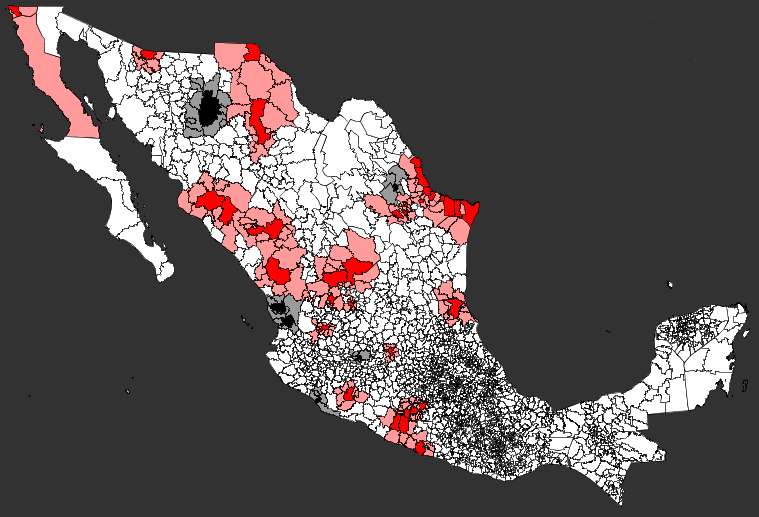
\includegraphics[scale=0.3]{Images/intervened.png}
			      \caption{\textbf{Red} (Black) = municipalities that received a military intervention. \newline
			\textbf{Pink} (Grey) = municipalities not directly intervened, but part of a treated region (neighbor to a red).\newline
			 \small{Black and Grey related to interventions in 2010 - we have no post intervention data}.}
			\label{treatedUnits}
			\end{figure}
			
			\item \emph{\textbf{No Hidden Value:}} It is important to have an unambiguous definition to identify treated units, and be clear about what potential outcomes we are comparing. Based on the Escalante paper, we defined \textbf{ Military intervention} as a confrontation between army and organized crime that resulted in at least 3 civilian deaths (where civilian could be a member of a cartel). The list we used was obtained from the paper in question. This list could be improved by scrapping newspapers and SEDENA press releases. We define \textbf{treatment} for a region as receiving at least one military intervention between 2007 and 2010.
			\begin{itemize}
				\item We define \textbf{Timing of treatment} for a region to be the first point in time in which a municipality in the region received an intervention.
			\end{itemize}  			
		\end{itemize}
		
\subsection{Unconfoundedness}			
	Unconfoundedness assumes we have all covariates, \textbf{X}, such that given \textbf{X},  treatment assignment is independent of \textbf{Y}. This is a critical untestable assumption. However, we have previously mentioned missing covariates that we believe are important but we do not have access to these in a reliable or time-relevant form. The covariates included in our study are displayed in Table \ref{Tab1}. Note that higher order effects involving Homicide Rate of 2006 at the municipality level were used in the propensity score.
		
	\begin{table}[htdp]
	    \footnotesize
	        \begin{center}
		\resizebox{10cm}{!}{  
	        \begin{tabular}{|l|l|l|}
	            \hline
		           & \multicolumn{2}{c|}{Background Covariates}\\
				Type&Municipality Level & State Level\\
	            \hline
	           \multirow{2}{*}{Demographics}&Homicide Rate 2006&Homicide Rate 2006 \\
		& Homicide Rate 2006 Class (above the mean) & \\
	 			&Population 2006&Population 2006 \\
				& Number of Criminal Rivalry Deaths & \\
				& (Dec 2006, Jan, Feb, Mar, Apr 2007) & \\
				\hline
				Economics&Income 2006 & GDP 2006\\
				\hline
				\multirow{2}{*}{Location}&Latitude&\\
					&	Longitude&\\
					\hline
					\multirow{3}{*}{Education}&Average Years Of Schooling&\\
						&Proportion that can read and write&\\
						&Proportion that speaks an indigenous language&\\
						\hline
					\multirow{2}{*}{Health}& Number of Doctors per medical unit&\\
						&Missingness indicator for the above&\\	
								            \hline				
				Politics&Political Party in power at the end of 2006 &\\
				\hline
				\multirow{2}{*}{Roads}& Longitude of Roads&\\
				& Missingness Indicator of above &\\	
	            \hline
	        \end{tabular}}
	    \end{center}
	    \caption{Covariates included}
	    \label{Tab1}
	\end{table}
	
\subsection{Estimand}
		        Let $Y_i(1)$ denote the homicide rate change in region $i$ from one year before to one year after receiving a military intervention, and $Y_i(0)$ what this difference would have been if it hadn't received it (Rubin Causal Model). Figure \ref{responseDef} displays a sketch of the potential outcomes, where $HR_i(0)$ and $HR_i(1)$ denote the homicide rate time series for region $i$ under control and treatment respectively, and $HR_i^{x}(1)$ denotes the homicide rate for region $i$ at the \emph{end} of year $x$.
		
		
				\begin{figure}[htdp]
					\centering
				      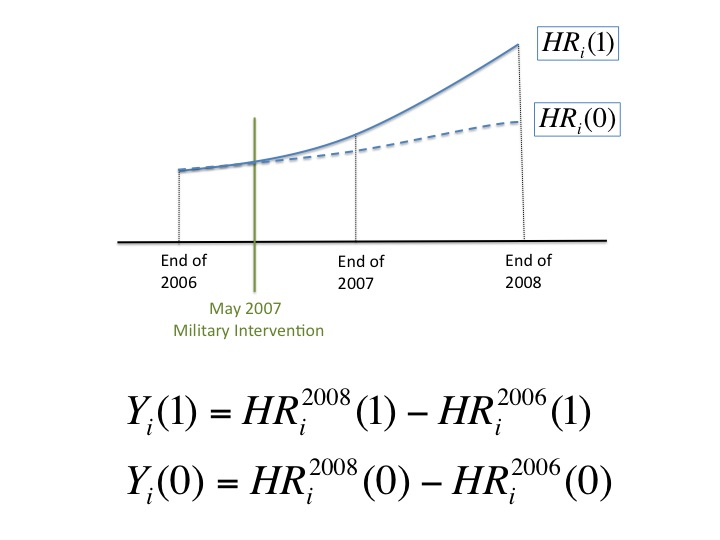
\includegraphics[scale=0.3]{Images/ResponseDef/Slide1.jpg}
				      \caption{Definition of the potential outcomes}
				\label{responseDef}
				\end{figure}
		  		Our \textbf{ main estimand} is the average causal effect of the military intervention, for the regions that could have been intervened. That is, $$\tau=\overline{Y}(1)-\overline{Y}(0)=\frac{ \sum_{i=1}^{N} Y_i(1)-Y_i(0)+ Y_{i'}(1)-Y_{i'}(0)}{2N},$$ where $N$ is the total number of such regions.
				\begin{itemize}
					   \item Let $N_i$ denote the number of municipalities that correspond to region $i$, $w_{ij}= \frac{\textrm{Pop}_{ij}}{\textrm{Pop}_{i}} \textrm{ and  }\textrm{Pop}_{i}= \sum_j^{N_i}\textrm{Pop}_{ij}$, then 
						$$Y_i(1) = \sum_{j=1}^{N_i}w_{ij}Y_{ij}(1) \textrm{ and } Y_i(0) = \sum_{j=1}^{N_i}w_{ij}Y_{ij}(0).$$						
				\end{itemize}
				Analogous estimands for two and three years post intervention are also of interest.
						\begin{table}[htdp]
							\centering
						\begin{minipage}[b]{0.3\linewidth}
						    \scriptsize 
					        %\begin{center}  
					        \begin{tabular}{|l|c|c|c|}
					            \hline
					            Region& unit& $Y_i(0)$&$Y_i(1)$\\
					            \hline
					            Ju\'{a}rez&1&$Y_1(0)$&$Y_1(1)$ \\
								 Ju\'{a}rez-like&$1'$&$Y_{1'}(0)$&$Y_{1'}(1)$ \\
								\hline
								Nogales&2&$Y_2(0)$&$Y_2(1)$ \\
								 	Nogales-like&$2'$&$Y_{2'}(0)$&$Y_{2'}(1)$ \\
								\hline
								\vdots&\vdots&\vdots&\vdots \\
								\hline
					            Apatzing\'{a}n&13&$Y_{13}(0)$&$Y_{13}(1)$ \\
								 Apatzing\'{a}n-like&$13'$&$Y_{{13}'}(0)$&$Y_{{13}'}(1)$  \\
					            \hline

					\end{tabular}
							%\end{center}
				\end{minipage}
				\hspace{2cm}
				\begin{minipage}[b]{0.3\linewidth}
						    \scriptsize
						        %\begin{center}  
						        \begin{tabular}{|l|c|c|c|c|c|}
						            \hline
						            Region& unit& $Y_i(0)$&$Y_i(1)$\\
						            \hline
						            Ju\'{a}rez&1&?&$Y_1(1)$ \\
									 Ju\'{a}rez-like&$1'$&$\hat{Y}_{1'}(0)$&? \\
									\hline
									Nogales-like&2&?&$Y_2(1)$ \\
										Nogales-like &$2'$&$\hat{Y}_{2'}(0)$&? \\
										\hline
									\vdots&\vdots&\vdots&\vdots \\
									\hline
						            Apatzing\'{a}n&13&?&$Y_{13}(1)$ \\
									 Apatzing\'{a}n-like&$13'$&$\hat{Y}_{13'}(0)$&? \\
						            \hline
						        \end{tabular}

						    %\end{center}
									\end{minipage}
									   \caption{Tables of all potential outcomes (left)  and of \emph{Observed-Estimated} potential outcomes (right).}
				    \label{Tab3}
				\end{table}
The subtable on the left of Table \ref{Tab3} shows all the quantities that we would like to know to reveal the TRUE value of the estimand. This is often called the SCIENCE in the Rubin Causal Model framework. The second part of this table is explained in the \emph{Estimation} section.					

\subsection{Matching method}
We used a combination of exact and propensity score matching. Three matches were found for each treated municipality. We \textbf{exactly matched} on Political Party in office at Municipality level in 2006, Homicide Rate 2006 Class (indicator for ``above the mean''), and Missing Indicator for Doctors per medical unit. The importance of 2006 is that it is the last year that is prior to all interventions listed. The selection of Propensity score was based on balance achieved. We considered
\begin{itemize}
	 \item all main effects
	\item higher order terms involving Homicide Rate 2006 at Municipality level
	\item log(Homicide Rate 2006 +1)
	\item log(State Homicide Rate 2006 +1)
	\item State Homicide Rate 2006$^2$
\end{itemize}

 

\begin{figure}[htdp]
    \centering
\subfigure[Arteaga, Coahuila (Guadalupe Region)]{
    \includegraphics[scale=0.45]{Images/ArteagaMatches.png}
	}
	\hspace{2cm}
	\subfigure[Concordia, Sinaloa (Sinaloa Region) ]{
	    \includegraphics[scale=0.3]{Images/ConcordiaMatches.png}
		}
\caption{Matched treated Municipality: Green, Matches: Blue}	
\end{figure}	


\subsection{Assessing Balance}
As in any observational study, balance in key covariates should be assessed before any analytical step. When a reasonable balance has been achieved, the design stage of the study ends and the analysis one begins. Readers should judge whether the balance achieved is enough for them to trust the results.  

Love plots are a very useful tool to evaluate balance. For this problem we had to come up with a reasonable understanding of what the baseline balance is. What we did for the initial balance was to impute the missing outcome for each treated municipality with the overall average of the control municipalities. Therefore the same value is used to impute the missing outcome for each treated region. Like the outcome, the covariate value for each treated region corresponds to a weighted average (based on population) of the municipalities that conform it. The plots displayed in Figure \ref{lpme} show a clear improvement with the 3 to 1 matching used. This is seen by the fact that the lighter, pointing upward triangles are closer to the vertical line on zero, which denotes no difference in the average values of the covariate between treated and control units. However, subfigure \ref{lpaddcovs} shows that the monthly total number of criminal rivalry related deaths before May 2007 (time of first intervention) was improved by a very small amount. However, we chose to focus on balancing the 2006 homicide rate reported by INEGI because those are the official data and it is unclear how reliable the criminal rivalry death count is. Also note these criminal rivalry covariates are not normalized by population. This information is not available at a monthly resolution.

\begin{figure}[htdp]
	\centering
	\subfigure[Main effects]{
       \includegraphics[scale=0.4]{Images/PQloveplot.pdf}
		}
		\subfigure[Additional covariates]{
	       \includegraphics[scale=0.4]{Images/PQloveplotExtraCov.pdf}
			\label{lpaddcovs}
			}
		\caption{Love plots}
		\label{lpme}
\end{figure}

Figure \ref{regionPS} shows the propensity scores by region. Keep in mind that the control regions (at the top) consist of three times as many municipalities as the intervened ones (at the bottom). And in some cases the number of municipalities is very low (e.g. Tijuana consists of 4). That said, the municipalities that look problematic are:
\begin{itemize}
	\item \textbf{Tijuana} because of the overlap in propensity score distributions. In other words, the propensity score values for the treated municipalities are above most of the values for the control ones.
	\item \textbf{Apatzing\'{a}n} and \textbf{Sinaloa} to a lesser extent because of the different shapes of the control and intervened histograms. 	
\end{itemize}	
\begin{figure}[htdp]
	\centering		
	        \includegraphics[scale=0.4]{Images/psByReg.pdf}
	\caption{Propensity score histogram by Region. Two histograms are displayed (vertically) for each region. Intervened regions are at the bottom, and control ones are on top.}
	\label{regionPS}
\end{figure}	
			
\section{Estimation}

The table on the right of Table \ref{Tab3} does not have only observed outcomes under ``control". That is the main difference between this problem and the ones which are usually set up in this framework. The outcomes of the controls are estimated using municipalities that were not intervened and that might not be neighboring to estimate what the homicide rate increase would have been for the treated municipalities conforming a region, which are in fact side by side. Doing this makes sense because in the absence of an intervention there is no reason to believe that there are spill over effects. However, we cannot conceive such a control region as receiving the same kind of intervention, because the municipalities in question are not neighboring. Therefore, the \emph{observed} outcome of the treated units is denoted by $Y_i(1)$, but the outcome of the control units is \emph{estimated}, and denoted by $\hat{Y}_i(0)$. 	

Let I denote the number of treated regions (here 13, 205 municipalities). Let $M_{ij}$ be the number of municipalities matched to the $j$th municipality in region $i$, and estimate $Y_{i'j}(0)$ and $Y_{i'}(0)$. Here $M_{ij}=3$.

      Let $\textrm{PopM}_{ij}=\sum_{k=1}^{M_{ij}}\textrm{PopM}_{ijk}$ be the sum of the populations of these matched municipalities. % this notation makes sense because these are matches to the jth municipality if tge jth region
 Then,
      $$\hat{Y}_{i'j}(0) =\sum_{k=1}^{M_{ij}}v_{ijk}Y^{obs}_{ijk}(0),\quad \quad \textrm{ where } v_{ijk}=\frac{\textrm{PopM}_{ijk}}{\textrm{PopM}_{ij}}.$$
      Therefore,
      $$\hat{Y}_{i'}(0) \quad =\quad \sum_{j=1}^{N_i}w_{ij}\hat{Y}_{i'j}(0)\quad =\quad\sum_{j=1}^{N_i}w_{ij}\sum_{k=1}^{M_{ij}}v_{ijk}Y^{obs}_{ijk}(0)\quad =\quad
      \sum_{j=1}^{N_i}\sum_{k=1}^{M_{ij}}\tilde{w}_{ijk}Y^{obs}_{ijk}(0) \quad \quad \textrm{ with } \tilde{w}_{ijk} = w_{ij}v_{ijk}, $$
      and
      $$\hat{\tau}=\frac{\sum_i^{I}[Y^{obs}_i(1) - \hat{Y}_{i'}(0)]}{I}=\overline{Y}^{obs}(1)-\overline{Y}^{est}(0).$$
      We know that $var(\hat{\tau})\leq var(\overline{Y}(1))+var(\overline{Y}(0))$, % add reference
and it achieves the bound under additivity of potential outcomes. We use estimates of the quantities on the right hand side of this equation to get a ``conservative'' estimate of the variance. Matching is often inexact, so that systematic differences in pre-treatment variables across the matched pairs may remain. For this reason the variance is usually estimated ignoring the pairs (in this case 3 controls are matched to each treated municipality). Again, this methodology diverges from the traditional one in the fact that the ``control'' regions can be formed from municipality matches \emph{that are not contiguous}. Therefore, \emph{artificial} matches are created (3 for each treated region), where the observed homicide rates of the control municipalities are weighted by the weights used for the treated region in question $w_{ij}$ in order to get an estimate for the homicide rate in the \emph{artificial} region. 

 % (Imbens Rubin on matched pairs) it attempts to find the control unit most comparable to the treated unit in all possible pre-treatment characteristics. Although in many cases making units comparable along observable dimensions need not be sufficient for obtaining credible causal comparisons, it is often a prerequisite for doing so. There are, however, two important differences between paired randomized experiments and matching in observational studies. The first is that in the latter case, unconfoundedness must be assumed—it is not guaranteed to be satisfied by design, as it is in a randomized experiment. Even when treated and control observations can be matched exactly on the observed covariates, there may exist unobservable factors that vary systematically between members of the same pair, affecting both their underlying probability of receiving the treatment, and their potential outcomes, and therefore creating biases. Thus inferences based on matched observational data are inherently less credible than those based on data from a paired randomized experiment. The second difference with paired randomized experiments is that . In


Now, \begin{eqnarray*}
  var(\hat{\overline{Y}}(0))&=&E(var(\hat{\overline{Y}}(0)|Y_i(0) \forall i'))+var(E(\hat{\overline{Y}}(0)|Y_i(0) \forall i'))
  =E\left(\sum var(\hat{Y}_i(0))/I\right)+\frac{var(\sum_iY_i(0))}{I}\\
\end{eqnarray*}
Now, $var(\hat{\overline{Y}}(1)) = S^2(1)/I$ because the all $Y_j(1)$ are observed.	

\subsection{Data Details}
There are 2456 municipalities, out of which 248 are classified as intervened. Of these 205 are classified as receiving an intervention prior to 2010 (a mixture of actually intervened municipalities and the neighboring regions). These 205 municipalities are grouped into 13 regions. The control pool consists of 2213 municipalities. 
			
\section{Results and Conclusion}
Table \ref{TabResults} and Figure \ref{figResults} show the results of our analysis. The regions are ordered in decreasing order of the of one year post intervention differences in the change of homicide rate. Understanding effectiveness as decreasing the violence (measured by homicide rate) the military interventions seem to have had a negative effect (increased homicide rate), although it is not significant. The Ju\'{a}rez region is a clear outlier, and it is the only region with an increase outside of the confidence band of the average effect. Apatzing\'{a}n is the only region with a decrease beyond the confidence band.  

\begin{table}[ht]
\begin{center}
			\resizebox{15cm}{!}{
\begin{tabular}{|l|rr|rr|rr|rr|}
  \hline
 Region& num of & Date of  & \multicolumn{2}{c|}{one year post intervention} &  \multicolumn{2}{c|}{two years post intervention}  &  \multicolumn{2}{c|}{three years post intervention}  \\ 
 & munis &  first int & $Y_i(1)$ & $\hat{\tau}_i$ (SD) & $Y_{2_i}(1)$ & $\hat{\tau}_{2_i}$ (SD) & $Y_{3_i}(1)$ & $\hat{\tau}_{2_i}$ (SD) \\ 
  \hline
Ju\'{a}rez & 16 & 2008 & 120.64 & 103.63 ( 4.52) & 203.69 & 173.51 ( 5.80) &  &   \\ 
  Tijuana & 4 & 2008 & 45.34 & 28.31 ( 9.81) & 48.20 & 41.49 ( 4.34) &  &    \\ 
  Acapulco & 36 & 2008 & 26.75 & 24.05 ( 3.92) & 25.24 & 15.06 ( 4.67) &  &    \\ 
  Guadalupe  & 20 & 2009 & 13.92 & 7.50 ( 6.45) &  &  &  &    \\ 
  Sinaloa  & 28 & 2007 & 11.67 & \textbf{4.66} ( 2.56) & 37.57 & \textbf{30.13} ( 4.33) & 64.43 & \textbf{41.56} ( 6.40) \\ 
  Te\'{u}l & 10 & 2009 & 5.65 & 2.88 ( 2.57) &  &  &  &   \\ 
  Celaya & 9 & 2009 & 5.25 & 2.82 ( 0.48) &  &  &  &    \\ 
  Villa de Cos & 22 & 2008 & 4.59 & 0.49 ( 5.01) & 6.07 & 2.00 ( 5.59) &  &    \\ 
  Nogales  & 6 & 2008 & 40.20 & -1.11 (16.97) & 75.91 & -7.50 (42.83) &  &  \\ 
  P\'{a}nuco & 14 & 2007 & -0.03 & \textbf{-1.83 }( 0.84) & 2.26 & \textbf{-1.65 }( 3.05) & 13.11 & \textbf{12.79} ( 1.29) \\ 
  Reynosa & 24 & 2008 & 4.85 & -3.24 ( 5.71) & 25.21 & 14.74 ( 5.37) &  &   \\ 
  Rinc\'{o}n de Romos & 7 & 2008 & -0.80 & -5.22 ( 0.62) & 0.37 & -4.46 ( 1.03) &  &  \\ 
  Apatzing\'{a}n & 9 & 2007 & -31.16 & \textbf{-26.44} ( 3.44) & -11.72 & \textbf{-21.94} (21.35) & -13.70 & \textbf{-7.03} ( 7.62) \\
\hline 
  $\hat{\tau}$ & 250 & - & 18.99 & 10.50 (12.35) & 31.75 & 18.57 (26.43) & 4.91 & 3.64 (25.27) \\ 
   \hline
\end{tabular}}
\caption{Estimated intervention effect. Yearly estimates were done independently.}
\label{TabResults}
\end{center}
\end{table}
Furthermore, if one looks at the estimates of the effects of those regions that have information available for more than one year post intervention assessment in Table \ref{}, it is clear that the tendency is to increase the homicide rates further the more time passes by. To this note, keep in mind that  
For your assessment of these results keep in mind that the main weaknesses of our analysis are that the Cartel information was not used, we did not achieve balance for criminal rivalry deaths, and we do not have a comprehensive list of interventions. Nevertheless, the lack of a comprehensive list would tend to decrease the difference in homicide rate. %(other intervened and dangerous regions would be incorrectly identified as controls)
 
\begin{figure}[htdp]
	\centering
  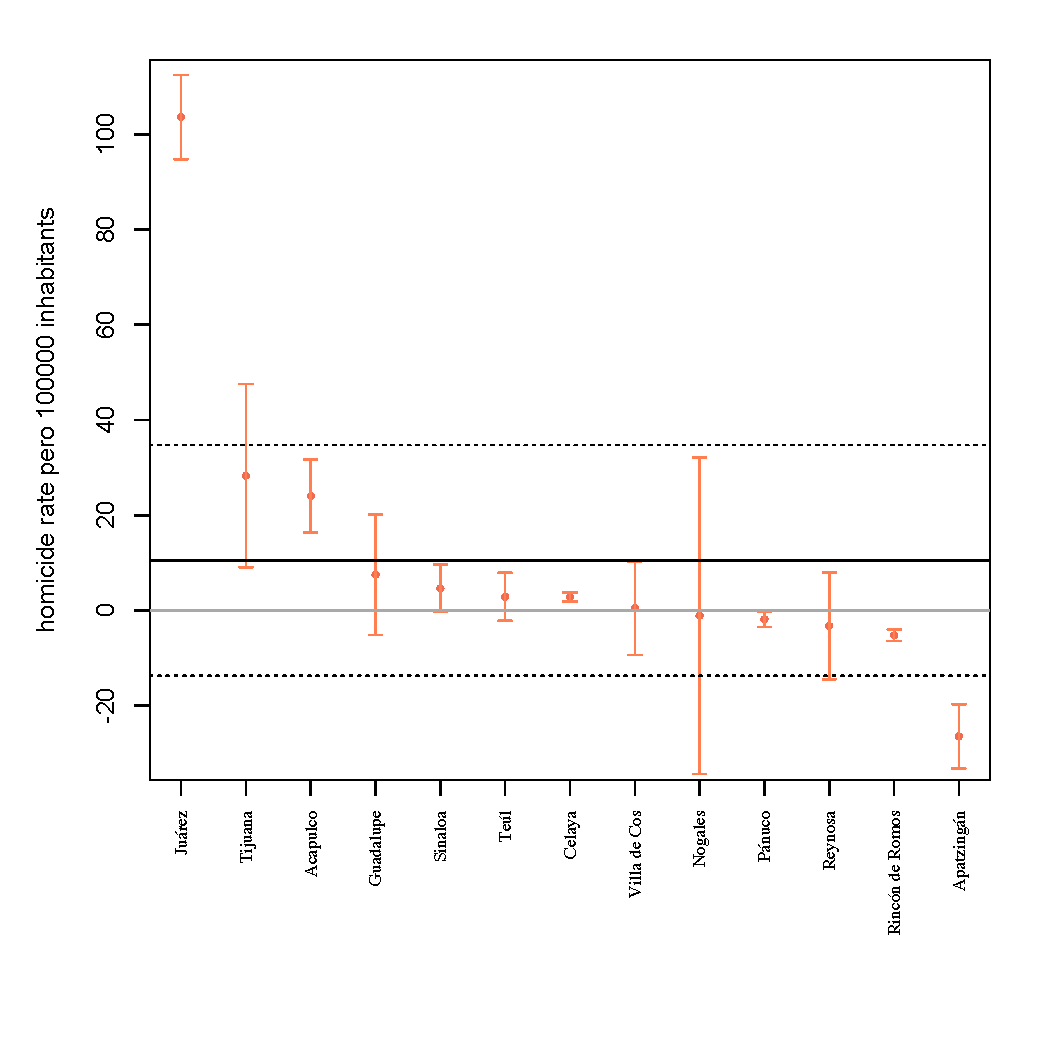
\includegraphics[scale=0.5]{Images/results.pdf}
  \caption{Results shown in decreasing order of differences in the change of homicide rate.}
\label{figResults}
\end{figure}



At the very least, this is a principled way of doing a conditional association study taking in to account very relevant covariates such as those listed in Table \label{Tab1}.

\section{Visualization}
An interactive visualization was created to be able to assess balance at the municipality, region and overall levels via loveplots. 

\section{Possible extension}
Estimate treatment effect with and without Ju\'{a}rez.
Use of cartel information before and after intervention as principal strata to try to get to the answer as to whether the decrease in 


        %\bibliographystyle{plain}
        \begin{thebibliography}{99}
          \bibitem{Abadie} Abadie, Diamond, Hainmueller  \emph{Synthetic Control Methods for Comparative Case Studies} (2009)
          \bibitem{NEXOS} Escalante F, \emph{Homicidios 2008-2009 La muerte tiene permiso} (2011)
          \bibitem{ImbensRubin} Imbens G. \& Rubin D.R., (2013)
          \bibitem{Rubin} Rubin D.R. ,\emph{Matched Sampling for Causal Effects},
\bibitem{Processing} Fry, B. and Reas, C., Processing Library for Visual Arts and Design
           \bibitem{Valle} Valle Diego (visualization and github) \url{https://github.com/diegovalle/Homicide-MX-Drug-War/blob/master/timelines/data/military-operations.yaml}
\bibitem{CRH}		Homicides attributed to criminal rivalry (2007-2010)
	\url{http://www.presidencia.gob.mx/base-de-datos-de-fallecimientos/}          
\end{thebibliography}

%%%% Get carreteras and índice de desigualdad for the municipalities. 
%%%% Also, recode the Homicide Rate in 2006 in to bins (maybe like caliper matching?) to improve balance
%%%% should we also include HR since 1990?
\end{document}